
\documentclass[a4paper,10pt]{report}
\usepackage{todonotes}
\usepackage[utf8x]{inputenc}

\usepackage[T1]{fontenc}

\usepackage{default}
\usepackage{amsmath}
\usepackage{enumerate}
\usepackage[]{natbib}
\usepackage{graphicx}
\usepackage{wrapfig} 


\makeatletter
\providecommand\phantomcaption{\caption@refstepcounter\@captype}
\makeatother

\bibpunct{(}{)}{,}{a}{,}{,}
\usepackage{lmodern}
\usepackage[colorlinks=true,urlcolor=black,citecolor=black,linkcolor=black,bookmarks=true]{hyperref}
\usepackage[french]{babel}

\usepackage[footnotesize]{caption}
\usepackage[font=scriptsize]{subfig}
\title{Auto-organisation dans un essaim d'agents autonomes: évolution de comportements spécialisés}
% \usepackage{figure}
% \makeatletter 
% \let\c@lofdepth\relax 
% \let\c@lotdepth\relax 
% \makeatother 

% \usepackage{subfig}
\captionsetup{figurewithin=none}  
\captionsetup{tablewithin=none}
% \usepackage{listings}
% \usepackage{float}
% \floatstyle{boxed} 
% \restylefloat{figure}
% \lstset{inputencoding=utf8x, extendedchars=\true}
%%%%%
%CF: titlepage.tex!!
%
\author{Simon Carrignon}
\date{9 Juin 2011, soutenu le 14 Juin 2011}
%\tiny École~Pratique~des~Hautes~Études, INRIA Saclay\\
% \includegraphics[height=0.5cm]{images/logo_ephe_large.jpg} %declare logo image with an alias here 
% \hspace{.5cm} \includegraphics[height=0.5cm]{images/logo_INRIA.png}\\% declare logo image with an alias here 
% }
% \date{\small Mémoire présenté en vue de l'obtention du Master de Cognition Naturelle et Artificielle\\
% Sous la responsablité scientifique de M. Nicolas Bredèche et sous la résponsabilité pédagogique de Mme Joëlle Provasi\\
% Rapporteur: Marc Bui, Joëlle Provasi\\
% Année académique 2010-2011}V
% \usepackage{tikz}
% \usetikzlibrary{decorations.pathreplacing}
% \logo{\includegraphics[height=0.5cm]{images/logo_ephe_large.jpg}}
% \title{Specialization in a swarm of robot using online, onboard, environment driven evolution\\ \vfill}
%%%%%


%%%%%%%
%!!!!!!!!!!!!!!!!!111
% VERSION UN PEU BIZARRE CAR PAS DERNIEre VERSION MAIS PRESQUE PUIs RETOUCHË POUR ENVOYER A DAUTRE QUE LES RAPPORTEURS!!!
%Version re-remise à jour (qui compile malgrès les erreurs) pour envoyer le 10 Décembre 2013 à R. Doursat. C'est quand même pas top top, et ça meriterait une relecture bien plus complête
%%%%
\usepackage{array}

\usepackage{algorithm}
\usepackage{algorithmic}
\bibpunct{(}{)}{,}{a}{,}{,}
\usepackage{makeidx}
% \addtolength{\voffset}{-1.5cm}
% \addtolength{\textheight}{2cm}
% \addtolength{\hoffset}{-2.25cm}
% \addtolength{\textwidth}{4.5cm} 
% \setlength{\columnsep}{.5cm}
% % % 	"free-ride" setup duration & 75 generations \\ 
\makeindex

\newenvironment{keywords}{\global
\noindent{{\bf{Keywords:}} }\ignorespaces
}


\begin{document}
\renewcommand{\abstractname}{Abstract/Résumé}
%%%
%TODO dans title page: Pb logos, etc

\begin{titlepage}
\Large

\noindentÉcole~Pratique~des~Hautes~Études\\
TAO/LRI\\
INRIA Saclay\\ %École~Pratique~des~Hautes~Études
 
 \vfil
 \includegraphics[height=1cm]{images/logo_ephe_large.jpg}
 \hfill \includegraphics[height=1cm]{images/logo_INRIA.png}% declare logo image with an alias here 
 
 \vfill
 
 
\begin{center}
 {\huge
\textbf{ 
	Auto-organisation dans un essaim d'agents autonomes : évolution de comportements spécialisés
	%\'{E}tude de l'emergence de spécialisation et speciation dans des populations d'agents autonomes artificiels via une évolution en ligne et embarqué non supervisé}
	}
 }
 \vfill
 
 Simon Carrignon 
 

\vfill 
 
{
	\normalsize Mémoire présenté en vue de l'obtention du Master de Cognition Naturelle et Artificielle\\
}
{
% 	\begin{flushleft}
	 \normalsize
	\vspace{.5cm}
	\noindent Sous la responsablité scientifique de M. Nicolas Bredèche\\ \noindent Sous la résponsabilité pédagogique de Mme Joëlle Provasi\\
% 
% 	\end{flushleft}

}
{	 
	\normalsize
	\vspace{.5cm}
	Rapporteurs : Marc Bui, Joëlle Provasi\\
	\vfill
}
 
 {\small Année académique 2010-2011 }
\end{center}
\end{titlepage}

%%
\tableofcontents

\listoffigures


\begin{abstract}
The aim of this study is to look at mechanism of specialisation and speciation through artificial and open-ended evolution. We want to see and caracterize how reacts a swarm of autonomous agents evolved through an on-board, on-line, unsupervised and environment-driven evolutionnary algorithm when the swarm needs to divide itself in two specialised, different subpopulation in order to allow the whole swarm to survive. Our goal is to show that specialisation of autonomous agent in unknown and unpredictable environment is possible using distributed and unsupervised evolution. We find that naturally an allopatric speciation emerges that allow two specialised species to survive during a certain amount of time, but that more environmental constraints should be implemented  to let sympatric speciation occurs. 

Le but de cette étude est d'observer les mécanismes de spécialisation et de spéciation à l'\oe uvre dans un algorithme d'évolution artificielle \emph{open-ended}. Nous cherchons à caractériser le comportement d'un essaim d'agents autonomes soumis à une évolution en ligne, embarquée, non supervisée et dirigée par l'environnement lorsque l'essaim doit se diviser en sous-populations spécialisées pour survivre dans sa totalité. Le but est de montrer que la spécialisation d'agents autonomes dans un environnement inconnu et imprévisible est possible à l'aide d'une évolution distribuée, embarquée et non supervisée. Nous montrons ici que naturellement un spécialisation allopatrique émerge, permettant la création et le maintient pendant un certain temps de deux espèces différentes mais que des contraintes environnementales plus fortes sont nécessaire pour maintenir cette spécialisation voir obtenir une spéciation sympatrique. 

\begin{itshape}
\paragraph{Keywords :}
Swarm Intelligence, Open-ended Evolution, Specialization, Artificial Evolution, Artificial Life, Sympatric Speciation, Allopatric Speciation, Evolutionary Robotics.

\end{itshape}

\end{abstract}

\chapter{Introduction}


% \section{Conception automatique de comportements robotiques}

Concevoir un contrôleur pour un robot est une tâche complexe et difficile. Il faut prendre en compte l'environnement, les caractéristiques matérielles, et ces paramètres sont tous susceptibles de changer. De plus il ne faut pas perdre de vue la tâche pour laquelle le robot a nécessairement été con\c cu et son \emph{objectif}. Une possibilité est de permettre au robot de s'adapter automatiquement et en ligne à ces variations paramétriques pour atteindre son but.

Pour réaliser de tels comportements auto-adaptatifs une solution est d'utiliser des techniques d'évolution artificielle. Celles-ci permettent d'adapter automatiquement et en ligne les contrôleurs des robots, en fonction du comportement que l'on souhaite obtenir. Mais dans certains cas ce comportement désiré peut être très difficile à définir, voir inconnu. C'est pourquoi il est parfois nécessaire d'appliquer une évolution \emph{open-ended}\footnote{\'{E}volution en \emph{boucle ouverte}, sans but prédéterminé. Nous continuerons à utiliser le terme anglais dans la suite du rapport}.

C'est l'étude de cette évolution \emph{open-ended}, appliquée à des essaims d'agents autonomes, qui nous intéresse ici. Plus particulièrement nous voulons voir si de tels systèmes sont capables de produire des populations spécialisées dans l'accomplissement de sous tâches différentes, et si oui quelles sont les conditions qui rendent possible cette spécialisation.

% en passant par des phénomènes proches de la spéciation que observable dans les systèmes biologiques. 

% 'e 
% Cette evolution artificielle s'appuie en générale sur d'
% Dans certains cas l'objectif même du robot est difficile à définir et susceptible de changer ;  p'

% 'e prendre en compte les environnements changeants et de produire des comportement auto-adaptatifs.


% , 'l'adaptation en ligne '''De nombreux paramètres sont à prendre en compte: l'environnement, les caractéristiques matérielles.  

% o
% Contrôler un robot est une chose complexe. 

% Concevoir un programme, un algorithme, pour contrôler un robot ou un groupe, un <<essaim>> de robots n'est pas une chose aisée.


% D'abord, et assez logiquement, contrôler un robot implique \emph{travailler avec} des robots ; qui sont des objets fragiles, chers et con\c cus par l'homme. Et si leur qualité ne cesse de s'améliorer, ils n'en demeurent pas moins, et resterons toujours à un certain degré, faillibles et imparfaits. La précision des capteurs est limitée et peut varier entre les capteurs d'un même robot, les moteurs ne sont jamais réglés à l'exact identique, les composants sont susceptibles de souffrir de l'usure du temps à des degrés variable, etc. 

% Ces imperfections matérielles obligent ingénieur à tester, vérifier et ajuster très souvent et avec précision les paramètres qu'il utilise pour régler son robot. 

% Si de surcroît l'environnent dans lequel sera amené à évoluer le robot est connu pour ses caprices ou pire, totalement inconnu, alors la tâche devient quasiment impossible. L'intérêt est donc de trouver des techniques permettant l'automatisation de la mise au point et du réglage de ces contrôleur. 

% \todo{integré swarm intelligence, approche reactive vs IA classique, }
%D'autant qu'à ces considérationss, qui portent sur la compléxité, la variabilité et l'incertitudes des données du monde extérieur per\c cues par un agent, s'ajoutent celles concernant la manipulation et la prises de décision associée à ces données. Comment le robot va-t-il et doit-il réagir\,? En fonction de ces donnée, quelles comportement adopté\,? Et pour ce faire dans des environnements complexes il est très difficile de manipulé des concept de haut niveau et de concerver beuaoup d'information au sujet du monde. En effet plus la quantité d'information augmente,, plus le ocup en calcul auggmetne, plus les traitement sont long,e tc... Ajjouter a cela le prix des robots, et vous comprendrez qu'il n'est pas possible d; utiliser les techniques appliquer pour battre les joueuer d'echec notre environnement étant en perpetuellement changement, nos robots, simpe et de capacité très limités. Cest pourquoi nous nous tournerons vers les des stratégie reactive, plus imple, basé sur l'intéraction direct entre l'agent et son environnement comme décrit par~\cite{braintenberg86vehicles,brooks91intelligencewithoutreason},\\ou pas
% De plus concevoir un robot qui réagie "bien" dans un grand nombre d'énvironenment et de situation est un probleme très complexe. Si l'on veut un robt ''

% Dans ces cas complexes, pourquoi ne pas chercher l'inspiration auprès de l'algorithme de conception d'agents autonomes le plus efficace, et aux résultats les plus aboutis jamais obtenus: \emph{l'évolution des organismes vivants}, où comme il est plus courant de l'appeler: \emph{la nature}. 

% En effet, dans la nature les agents autonomes, qui sont l'ensemble des êtres vivants \footnote{Même si la définition d'être vivants est bien probablement sujet à débat et mériterait qu'on si attarde.}, évoluent et s'adaptent directement dans l'environnement avec lequel ils interagissent, sans supervision extérieure aucune \footnote{En excluant le cas insoluble de Dieu et autres entités supérieures}, et sont ainsi capable d'ajuster leurs comportements en fonction direct de l'environnement. 

% \section{ Spécialisation de sous-populations évoluant dans des environnements changeant}

% Et comme nous allons le voir, de nombreux systèmes d'évolution artificielle ont été conçus en s'inspirant de cette nature et «implémentent» une évolution \emph{open-ended\footnote{\'{E}volution en \emph{boucle ouverte}, sans but prédéterminé. Nous continuerons à utiliser le terme anglais dans la suite du rapport}}, aussi proche que possible de l'évolution naturelle, et à l'instar de laquelle les organismes évoluent en continue (\emph{onlive}) au sein même de l'environnement dans lequel ils doivent survivre (\emph{onboard} ou \emph{embedded}), et ce sans aucune intervention extérieur (\emph{unsupervised}). 


% C'est l'étude de ces systèmes qui nous intéresse ici. Et plus particulièrement leurs réactions lorsque l'environnement nécessite la spécialisation des individus qui l'occupent. Notre but est d'observer comment un système d'évolution artificielle dans lequel doivent survivre des essaims d'agents autonomes, peut spécialiser des sous-populations de ces essaims...\todo{partie a revoir conceptuellement}


Ce rapport commence par situer le cadre du projet en reprenant les principes et concepts des approches choisies (Chapitre~\ref{ch:context}), soit: l'évolution \emph{open-ended} d'essaims d'agents autonomes au sein d'environnements dans lesquels l'émergence de spécialisation est nécessaire pour la survie de l'essaim. Suite à quoi nous expliquerons les techniques et méthodes utilisées pour observer ces comportements ainsi que les caractéristiques des expériences menées (Chapitre~\ref{ch:materiel}). Pour terminer nous présenterons et analyserons les résultats obtenus suite aux expériences (Chapitre~\ref{ch:result}), et discuterons de fa\c con plus général du projet, sur ces implications et sur les questions qu'il soulève et auxquelles il faudra répondre par la suite (Chapitre~\ref{ch:discussion}).


\chapter{Contexte et motivations }\label{ch:context}

Entre vie artificielle et robotique évolutionnaire, notre approche se veut bio-inspirée, avec pour buts étudier et permettre la spécialisation et la spéciation (cf.~\ref{sec:concept:speciat}) de larges groupes de robots aux comportements et capacités simples \citep{brooks91intelligencewithoutreason}, qui évoluent artificiellement directement dans leur environnement et sans aucune supervision. Ce chapitre introduit ces concepts et approches utilisés (\ref{sec:concepts}) ainsi que les principes généraux des phénomènes étudiés (\ref{sec:special}).


\section{Des essaims d'agents autonomes soumis à une évolution \emph{Open Ended}}
\label{sec:concepts}
%\subsection{Trouver des solutions pour des problèmes complexes}\label{sec:prob}
%%%%LISTING DES PROBLEMS RENCONTRÉS EN ROBOTIQUE
%intelligence artificielle classique et recherche operationnelle très difficile à mettre en oeuvre dans le cas d'environnement changement, les ressources avec de tres grand nombre d'interaction robot/environnement robot/robot, espace de recherche de solutions trop vaste et demande en cacul trop importante. D'autant que bien souvent les solution materielles sont limitée et les puissances de calculs relativement faible pour permettre des comportement adéquat lrosqu'il est necesaire de ne serait-ce que longer des murs et eviter des obstacle. Les solutions de recherches operationnelles classique (astar, etc...) sont inffeicace. De plus les environnement ne sont pas connus et change de facon dynamique parfois en fonction meme du comportement des agents ; ce qui rends la notation (le calcul d'une \emph{fitness} ) quasiment impossible rapport
Notre étude porte sur des essaims d'agents autonomes aux capacités simples, limitées, dont les comportement évolueront sans être supervisés.

Nous utilisons le terme d'agent autonome définit comme <<un système incarné et parti intégrante d'un environnement qu'il peut sentir et sur lequel il peut agir>>  %dans le but d'accomplir ses objectif et de à modifier ses perceptions future>> 
~\citep{franklin97autonomousagent}, en faisant abstraction du type d'environnement et de système, notre démarche se voulant indépendante des solutions matériel. Néanmoins notre optique à plus ou moins long terme est de valider les modèles obtenus en simulation sur des modèles robotiques ; c'est pourquoi parfois le terme de robot peut être employé pour remplacer celui d'agents ; nos agents étant modélisés de pour correspondre au mieux à certains modèles robotiques (voir section~\ref{sec:detailsdimple} ), mais ces robots ne sont qu'une \emph{instance} (un cas particulier) des agents autonomes (en anglais \emph{embodied agents}). 



\subsection{Swarm intelligence }
\label{sec:swarm}


\index{swarm intelligence}
\index{intelligence en essaim}

L'intelligence en essaim~\citep{garnier07biolprinswarinte} ou en anglais \emph{swarm intelligence}, est née de l'observation par les biologistes des organismes vivants organisés en colonies, essaims, bancs et autres groupements sociaux de taille et d'envergure variable. 
Que ce soient les fourmis, les abeilles, certains poissons ou l'étrange \emph{rat taupe}, ces espèces comptent toutes sur la force de l'auto-organisation et de l'auto-adaptation qui émergent des interactions locales et multiples entre les différents individus qui composent ces colonies ainsi que les interactions entre ces mêmes individus et leur environnement.

\begin{figure}[H]
\centering
\includegraphics[width=.5\textwidth]{images/381340_9806}
\end{figure}



L'intelligence ici, au sens de <<capacité de traitement de l'information et réaction adapté en conséquence>>, ne naît pas de la puissance de calcul d'une entité centrale capable de stocker, de manipuler et de s'adapter à un grand nombre de situations, mais \emph{émerge} du parallélisme et de la distribution de tâches simples. La complexité des comportements globaux observables à l'échelle de la colonie, ne reflète en rien la simplicité des comportements locaux observés aux niveau de l'individu composant le groupe~\citep{detrain2002complexity}. 

Ces phénomènes d'auto-organisation allient de nombreuses qualités très recherchées par les concepteurs de contrôleur robotique:  \emph{la redondance}, \emph{l'adaptabilité}, la \emph{flexibilité}, \emph{la robustesse}, et l'utilisation d'agents simples, sans besoin calculatoire d'envergure, de capacité de stockage ou de matériel complexe, puissant et coûteux. C'est pourquoi ces systèmes intéressent tant les chercheurs qui les étudient donc en profondeur, que ce soit directement dans la nature~\citep{garnier07biolprinswarinte}, ou comme nous le ferons dans la suite de ce manuscrit, à travers des systèmes artificiels qui essayent d'en implémenter les caractéristiques~\citep{bonabeau99swarmintelligence,bonabeau97adaptivetaskallocationinspiredbymodeldivisionlaborsocialinsects,sumpter10collanimbeha}.

% Voici donc le type de populations dont nous allons observer artificiellement l'évolution, en comptant sur les propriétés de cette \emph{swarm intelligence} pour offrir la flexibilité et l'adaptabilité nécessaire afin que sans supervision, évoluent spontanément des sous-populations spécialisées.


\subsection{\'{E}volution artificielle \emph{open-ended}}
\index{évolution artificielle}
\index{évolution open-ended}
\index{algorithme génétique}

\label{sec:oee}
Ajuster au mieux de multiples paramètres associés à des capteurs dont on ne connaît pas la précision à priori, sur des robots aux caractéristiques différentes, est une tâche souvent complexe qu'on peut souhaiter d'automatiser. 

Une solution est d'utiliser l'idée simple proposé par \cite{holland1975adapnatuartisystintrappltobiolcontartiinte} avec les algorithmes génétiques. Si parfois, trouver une solution ou l'ajustement précis de paramètres multiples et variables dans des systèmes informatiques peut être est très difficile et prendre un temps trop important, laissons faire le hasard et un zeste de sélection. Suivons l'exemple de la nature, choisissons au hasard des architectures, des solutions et sélectionnons les meilleures, modifions ces meilleures et recommen\c cons, jusqu'à satisfaction. 

% C'est ainsi  que, reprenant ces principes qui ont changé notre vision du monde il y a presque deux siècles lorsque~\cite{darwin59originspeciesbymeansnaturalselectionorpreservationfavouredracesstrugglelife} les énonçait, les informaticiens ont pu utiliser à leur profit les forces de l'évolution.

% Ces techniques ont trouvé très vite des applications aussi diverses que fructueuses dans à peu près touts les domaines de l'informatique. 


Dans le cadre de la robotique, l'utilité de telles stratégies permettant de répondre en partie aux problèmes de la conception automatique de contrôleurs évoquée en introduction, a rapidement été mise à profit par ce qu'il est convenu aujourd'hui d'appeler, la \emph{robotique évolutionnaire}~\citep{nolfi00evolrobobiolintetechselfmach}.
À défaut de trouver la bonne fa\c con de coder tous les paramètres pour permettre au robot d'avancer sans s'écraser sur le premier mur venu, au moins sommes nous capables de voir (ou d'entendre) le robot au moment de l'impact ; et donc en mesure de dire que ce n'est pas vraiment la solution la mieux adaptée.  Mais subsiste un problème, déjà soulevé en introduction: il est malheureusement nécessaire d'être, <<en mesure de dire que ce n'est pas vraiment une bonne solution>>.

Parallèlement de nombreux chercheurs en vie artificielle ont exploré la voie de l'évolution \emph{open-end}~\citep{ray91tierra,adami94avida}, et poussé plus loin encore la bio-inspiration. Cette fois-ci plus question de \emph{sélectionner} en attribuant une qualité aux individus observés. L'unique but est d'\emph{observer} l'évolution des individus au sein de l'environnement. D'observer les réactions du système, selon les contraintes de l'environnement, les capacités des agents, sans intervenir d'aucune fa\c con.

Cette étude de l'évolution \emph{open-ended} est partie intégrante des grands défis des chercheurs en Vie Artificielle~\citep{bedau00openprobartilife} qui font ainsi passer l'évolution du statut d'outils à celui d'objet d'étude.
Le but est de trouver: (a) \emph{ce qui est inévitable dans l'évolution de la vie},(b) \emph{les caractéristiques communes à tous les processus évolutionnaires}, et pour finir, ce qui nous intéresse plus particulièrement dans le cadre de cette étude: (c) \emph{trouver les conditions minimales d'évolution pour passer de systèmes répondants uniquement à des environnements simples et spécifiques, à des systèmes capables de généraliser et répondre dans de multiples environnement}~\citep[voir respectivement les chapitres 3.6, 3.10 et 3.7 ]{bedau00openprobartilife}.

Maîtriser ces systèmes \emph{open-ended} permettrait de bénéficier des avantages des techniques évolutionnaires classiques (auto-adaptation et design automatique) tout en s'affranchissant de la nécessitée de connaître \emph{a priori} les comportement recherchés.

Ce qui nous intéresse plus particulièrement dans cette étude est de savoir comment ces systèmes d'évolution \emph{open-ended} se comportent lorsqu'ils doivent permettre la spécialisation des populations qui évoluent en leur sein?
Quelles caractéristiques doivent posséder de tels systèmes pour que cette spécialisation ait lieu?

%De plus l'évolution open-ended partage de nombreux points commun avec l'embodied evolution~\cite{watson02emboevoldistevolalgopopurobo}. Qui permets de distribuer le mécanisme d'volution




\section{Spécialisation et Spéciation}

Souvent pour exploiter un environnement donné, ou pour qu'un groupe d'individus accomplisse une tâche efficacement, il est nécessaire que les entités qui composent le groupe ou la population se spécialisent. Dans la nature cette exigence peut être satisfaite soit par la division du travail au sein d'une même espèces, soit par la spéciation des organismes vivants en de multiples espèces spécialisées dans l'exploitation de ressources et de niches écologiques différentes.
\label{sec:concept:ssl}

\subsection{Spécialisation}
\index{spécialisation}
\label{sec:concept:special}

La spécialisation est un phénomène complexe observable à de nombreux niveaux dans la nature. Des modèles de spécialisation comportementale observés dans la nature chez les insectes sociaux par exemple~\citep{bonabeau96quantitativestudyfixedthresholdmodelregulationdivisionlabourinsectsocieties}, à la division du travail chez l'homme~\citep{smith1776wealthofnation} jusqu'aux cellules spécialisées des organismes pluricellulaires, elle permettrait dans bien des cas une gestion et une utilisation optimale de l'environnement.
% Ainsi étudier les mécanismes qui permettent son émergence, en comprendre les causes et les pendants évolutionnaires, est un défis d'un importance capitale.

% Les modèles artificielles si interresent aussi beaucoup et~\cite{}
Comprendre ces mécanismes pourrait permettre de comprendre comment l'évolution a réussi à produire une si grande richesse, exploitant toutes les ressources disponible en distribuant chaque espèce au mieux. Et comprendre permettrait d'adapter et utiliser ces mécanismes sur des essaims de robots et autres modèles artificiel, pour obtenir des systèmes capable de se spécialisé automatiquement et de la meilleur façon qu'il soit. C'est pourquoi un nombre importtant de travaux depuis une 20aine d'années portent sur l'étude des détails de cette spécialisation.

Optant pour des approches diverses, beaucoup de chercheurs ont exploré comme nous la voie de la spécialisation en reprenant les techniques des essaim biologique que nous avons présenté en~\ref{sec:swarm}~\citep[pour une revue complète de ces études utilisant l'approche \emph{swarm intelligence} et des questions qu'elles soulèvent voir:][]{nitschke08emergentspecializationbiologicallyinspiredcollectivebehaviorsystems}.


% ' comment maîtriser les mécanismes évolutionnaires à l'\oe uvre dans les systèmes \emph{open-ended} pour que cette spécialisation d'essaim d'agents autonomes émerge ?

% mais peut l'on fait par le biais d'une évolution \emph{open-ended} (cf.~\ref{sec:oee}), la spécialisation s'obtenant par la spéciation des groupes évolués.

\subsection{Spéciation}
\label{sec:concept:speciat}

Dans la nature, un des moyen les plus observé pour obtenir cette spécialisation reste la spéciation: est-il possible d'observer cette spéciation dans des essaims d'agents autonomes soumis à une évolution \emph{open-ended}?

\index{spéciation}
En biologie la spéciation est le phénomène qui entraîne la séparation d'une espèce donnée en deux sous espèces au caractéristiques différentes et ne pouvant plus échanger de matériel génétique. Elle peut parfois permettre à une population initiale de s'adapter à la pression environnementale en la séparant en deux espèces spécialisés capable de tirer un profit maximum de l'environnement.


\begin{figure}[H]
\centering
\subfloat[Allopatrique] {\label{fig:specAl} \includegraphics[width=.3\textwidth]{images/SpeciationAl}}
\hfil
\subfloat[Sympatrique] {\label{figa:specSy} \includegraphics[width=.3\textwidth]{images/SpeciationSy}}

\caption{Les deux principaux types de spéciation}
\label{fig:speciation}
\end{figure}


Plusieurs théories associées à différents cas de figure permettent d'expliquer les raison de cette spéciation:

La \emph{spéciation allopatrique} (figure~\ref{fig:specAl}), \index{spéciation allopatrique} classiquement attribuée à~\cite{mayr1942systematics} est la plus courante et la mieux connue. Dans ce cas de figure la population est coupée en deux par une contraintes géographique/géophysique: une montagne, un glissement de terrain, vient séparer une colonies d'insectes en deux sous-population qui évoluent ensuite séparément. S'écoulent les siècles et dérivent les génomes, tant qu'à la réunion des deux sous-colonies, les chances sont fortes pour que la dérive génétique ait rendu les deux populations suffisamment distinctes pour en faire deux nouvelles espèces.
\index{spéciation allopatrique}

La \emph{spéciation sympatrique} (figure~\ref{figa:specSy}), \index{spéciation sympatrique} en revanche, a lieu alors que les deux sous-populations continuent d'interagir et de se côtoyer. Dans ce cas la spéciation est plus complexe à analyser et ne peut être due à la simple dérive génétique. Malheureusement les données sont difficiles à récolter et aujourd'hui encore les théories divergent, sont nombreuses et encore largement controversées et sujettes à débats. Mais des études la mettant en avant et témoignant de sa faisabilité théorique ont vu le jours~\citep{geritz97evolutionarilysingularstrategiesadaptivegrowthbranchingevolutionarytree,dieckmann99originspeciesbysympatricspeciation}
, parfois même appliqués avec succès à des modèles artificiels d'évolution~\citep{holmgren07artificialneuralnetworksmodelsspecializationguildevolutionsympatricspeciation}. L'intérêt de ce type de spéciation est pour nous primordial puisque les individus de notre population de robots doivent, dans l'idéal, pouvoir continuer à interagir entre eux sans pour autant perdre leur spécialisation.
\index{spéciation sympatrique}



%TODO
%  Obtenir une specialisation en utilisant les méthodes présentées en~\ref{sec:swarm} et en~\ref{sec:oee} permettrait de s'affranchir des nombreux problèmes mise en avant en  introduction. L'idée est d'observer si des mécanimes de spécialisation sont à l'euvre lors de l'évolution open-endedd'essaims de robots dont la réaaction est bvasée sur un grand nombre d'intéraction entre des agents aux comportements simple, designer automoatique par evolution open-ended. 
% \cite{prieto10openevolasmeantoselfhetemultsystrealtime} ont déjà utliisé une évolution \emph{open-ended} dans des but à peu près similaires ; mais malgré le titre, leur évolution necessite un opérateru de séléction bien plus complexe que le notre!!
% \todo{ a deplacer et peaufiner}
%TODO

Comment donc réagissent des essaims d'agents autonomes, lorsqu'ils sont amenés à évoluer de fa\c con \emph{open-ended}, non supervisé, et en direct et que ces phénomènes de spéciation sont à l'\oe uvre? 

Quelles caractéristiques doivent posséder de tel systèmes pour qu'une spéciation de sous-population spécialisées ait lieu?

Voici les questions sur lesquelles nous allons nous pencher.

\chapter{Matériel et méthodes }\label{ch:materiel}


Dans cette étude nous allons observer l'évolution en ligne, distribuée et non supervisée de groupes d'agents autonomes, et analyser la nature de l'auto-adaptation dans le cadre d'un algorithme précis décrit dans ce chapitre.

Nous commencerons ici par présenter l'algorithme en question (mEDEA) et les questions et observations que son utilisation a soulevées dans des expériences déjà faite où apparaissent des sous-populations spécialisées. Nous terminerons ensuite par la description de l'environnement con\c cu et utilisé dans cette présente étude et des expériences mises au points pour étudier les mécanismes de spécialisation et de spéciation.


\section{\'{E}volution artificielle embarquée, distribuée et non supervisée }
\label{sec:algo}



\subsection{mEDEA \citep{bredeche11mcmds}}
Un système d'évolution \emph{open-ended} comme nous les avons décrit dans la parti~\ref{sec:oee}, doit permettre à un ensemble d'agents autonomes, aux caractéristiques techniques simple et relativement limitées, d'évoluer sans besoin de contrôle ni supervision humaine. Nous avons choisi pour cela un algorithme d'évolution embarqué, dans lequel l'évolution se fait par la sélection aléatoire des génomes capable de fournir aux robots les comportement les mieux adaptés dans un environnement donné. 
Cet algorithme, appelé mEDEA (pour minimal Environment-Driven Distributed Evolutionary Adaptation) et décrit par \cite{bredeche11mcmds} reprend à la lettre la métaphore du gène égoïste de \cite{dawkins76selfishgene} : chaque génome est perçu comme l'entité évolutive de base, qui utilise les robots comme <<outils>> pour se multiplier et se transmettre dans la population et à travers les générations.

\index{mEDEA}

Cet algorithme tourne en continue, parallèlement à une fonction de communication dont le but est de recevoir et stocker les génomes dans une Liste de Génomes Importés.

À chaque itération de la simulation, le comportement d'un agent donné est déterminé par une architecture de contrôle dont les paramètres sont stocké dans un génome actif, qui restera le même toute la durée d'une génération. Ce génome est émis en continue par la fonction de communication dans le rayon d'émission (limitée) du robot.

De fait algorithme implémente un certain nombre de caractéristiques simples mais néanmoins importantes de la structure traditionnelle des algorithmes évolutionnaires:

\textbf{Un opérateur de sélection }: c'est ici une simple sélection aléatoire d'un génome parmi la liste des génomes importés. Il n'y a aucune pression de sélection au \emph{niveau local de l'individu}.  Du point de vue de ce dernier, la sélection se fait totalement aléatoirement. Aucune entité centrale et aucune connaissance quelconque n'ai nécessaire pour sélectionner le génome  qui sera utilisé à la prochaine génération. La pression à la sélection n'est perceptible qu'à \emph{un niveau global},\emph{de la population}: plus un génome est distribué à un grand nombre d'individus, plus il se propage dans la population, plus il a de chance d'être sélectionner aléatoirement à la génération suivante \emph{en moyenne} dans l'ensemble de la population. De fait, plus larges sont les populations et les chances de croisements (au sens de rencontre et non génétique) entre les individus, plus précise et plus juste est la pression de sélection au niveau de la population.

\textbf{Un opérateur de variation (mutation)}: qui est assumé comme conservateur dans notre cas, afin d'assurer une continuité tout au long de la course évolutionnaire. Générer des copies modifiées d'un génome ne fait sens que si il existe une continuité dans la généalogie de ce génome: si il n'y a pas de variation l'algorithme finira par converger en moyenne vers la solution la plus efficace au sein de la population initiale. Dans les expériences que nous décrirons ensuite, nous opterons pour un opérateur aléatoire gaussien, inspiré par les Stratégies \'{E}volutionnaires~\cite{Beyer2002Evolution-strat}, avec laquelle l'ampleur des mutations locales peut être ajusté simplement à l'aide d'un paramètre $\sigma$.

\textbf{Un opérateur de remplacement}: en dernier lieu s'exécute un opérateur de remplacement, qui va décider de la <<mort>>, de la disparition des génomes remplacés. Ce remplacement se fait par (1) une délétion du génome actif, et (2), une sélection d'un génome au hasard dans la liste des génomes. Au niveau de la population, cela implique que les génomes survivants à une génération $G$ ont de fortes chances d'être corrélés avec des stratégies efficaces pour favoriser les rencontres du fait qu'un génome donné ne peut survivre qu'à travers des copies légèrement différentes de lui même transmises à d'autres robots tout au long de l'expérience.

Par sa définition, l'opérateur de remplacement fait que si, à la fin d'une génération, un robot n'a put recevoir de génomes (ou dit autrement, si un génome n'a pas été en mesure de contrôler un robot pour lui permettre de recevoir d'autre génomes) et que sa liste de génomes importés est vide, le robots ne sera plus en mesure de se déplacer. Il est ainsi mis en mode <<pause>>, et ne fait qu'<<écouter>>. 

La figure~\ref{fig:medeaRun} permets de voir à l'aide d'un exemple simple les différentes étapes de l'exécution de mEDEA. Les détails complets de l'algorithme sont disponibles en annexe dans le tableau~\ref{alg:medea}. 


% Une execution de ces différents opérateur actions et expliqué visuellement sur dans la figure~\ref{fig:medeaRun} 


\begin{figure}[H]
\centering
\newcommand{\imagesize}{5cm}
\subfloat[Step 1 : chaque robot est initialisé avec un génome aléatoire, représenté par une couleur différente et peut émettre ce génome et en recevoir d'autres de tout les robots à l'intérieur du cercle en pointillé (qui délimite en fait la distance d'émission maximale de la fonction de communication).]
{ \label{fig:medeastep0} \includegraphics[width=\imagesize]{images/medea0}}
\hspace{.1cm}
\subfloat[Step 2 : les robots se déplacent selon les règles établies par leur génome actif. Les robots avec les génomes vert et rouge échangent leur génome qui sont stockés dans leur liste respective.]
{ \label{fig:medeastep1} \includegraphics[width=\imagesize]{images/medea1}}\\

\subfloat[Step 3 : les robots continuent de se déplacer, cette fois les robots rouge et bleu échangent leur génome.]{ \label{fig:medeastep2} \includegraphics[width=\imagesize]{images/medea2}}
\hspace{.1cm}
\subfloat[Step 4 : les robots se déplacent mais aucun échange de génomes n'a lieu. Les génomes actifs ayant servis pendant les trois étapes précédentes sont supprimés et un autre est choisi aléatoirement parmi ceux recueillis dans la liste. Il sera muté puis utilisé comme contrôleur aux itérations suivantes jusqu'à la prochaine génération.]{ \label{fig:medeastep3} \includegraphics[width=\imagesize]{images/medea3}}

\caption[Illustration de l'exécution de mEDEA]{\ref{fig:medeastep0} Les trois robots sont initialisés avec un génome aléatoire représentés par trois couleurs différentes.  \`{A} chaque itération les robots se déplacent. Lorsqu'ils se croisent et que la portée des émetteurs le permet, ils échangent leur génome, qui sont ajoutés dans leur \emph{liste de génomes} (représentées par les tableaux en bas à droite de chaque image). \`{A} la fin de la génération (ici l'étape \ref{fig:medeastep3}) les robots sélectionnent aléatoirement un génome parmi les génomes présents dans leur liste et oublient le génome utilisé précédemment.
}
\label{fig:medeaRun}
\end{figure}

Ainsi, et comme le montre la figure~\ref{fig:medeaRun}, les génomes qui fournissent au robot le plus de chances de rencontrer beaucoup d'autres robots auront plus de chances d'être sélectionnés par la suite et d'être transmis aux générations suivantes. On le voit dans la figure \ref{fig:medeastep3}, le génome rouge a permis au robot sur lequel il était actif de rencontrer deux autres robots. Une copie de celui-ci sera \emph{forcement} sélectionnée à la prochaine génération puisque les robots vert et bleu n'ont que ce génome dans le liste. Deux versions légèrement modifiées de ce génome rouge contrôlerons donc des robots à la prochaine génération. En revanche, le génome bleu n'a pas permis au robots de s'éloigner du mur et n'aura qu'une chance sur deux d'être sélectionner ; tout comme le génome vert. Cela illustre bien qu'en moyenne, les génomes mieux adaptés à l'environnement auront plus de chances d'être sélectionner et ainsi soumis au processus évolutionnaire.


% \subsubsection{Caractéristiques des agents}

\subsection{Implémentations des comportements et observations préliminaires}
% \todo{trouver mieux}%TODO


\subsubsection{Détails d'implémentation}
\label{sec:detailsdimple}
Les agents sont modélisés sur la base des robots classiquement utilisés par les chercheurs en robotique, de type robots ePuck ou Khepera III \footnote{fabriqués respectivement par l'EPFL (\url{http://www.e-puck.org/}) et K-team (\url{http://www.k-team.com})}. Ils possèdent 8 senseurs de proximité (senseurs infrarouges dans les robots vendus sur le marchés) disposés autour du corps de l'agent et deux moteurs. Un moteur permet de définir la vitesse de translation et l'autre moteur permet de définir la vitesse de rotation.

Le contrôle de ces agents est laissé à un simple réseau de neurones artificiel multicouches \emph{MLP, Multi Layer Perceptron} non récurant très largement utilisé dans les expériences en robotique. Les détails d'implémentation (nombres de neurones, couches cachées, etc.) de ce réseau de neurones sont fournis dans la table~\ref{tab:params1} en annexe. 

% Il est à noté que notre étude ne porte en aucun cas sur l'étude des réseaux de neurones et 
Il ne faut pas perdre de vue que le cadre de notre étude se veut indépendant du contrôleur utilisé et que le choix d'un réseaux de neurone de ce type n'est du qu'à sa simplicité à son utilisé répandue en robotique et notamment en la robotique évolutionnaire.

Dans mEDEA le génome du robot sera donc composé des poids du réseau de neurones, et c'est le vecteur stockant les valeurs de ces poids que l'algorithme va muter. De plus et comme énoncé dans la partie précédente, des techniques inspirés de~\cite{Beyer2002Evolution-strat} sont utilisées pour mettre à jours les génomes et maîtriser leur variabilité.

La figure~\ref{fig:robotsbeha} montre deux exemples de comportements obtenus dans deux environnements différents dans lesquels est utilisé l'algorithme mEDEA. Dans un premier cas (Figure~\ref{fig:robotsbeha:A}) les robots doivent simplement avoir des gènes dans leur liste de gènes à la fin d'une génération pour pouvoir continuer à se mouvoir, dans le second cas (Figure~\ref{fig:robotsbeha:E}) les robots doivent en plus récupérer de l'énergie aux points d'énergie en orange sur les schémas. On peut noter la différence de comportements obtenus : dans le second cas les agents semblent bien <<naviguer>> de source en source et parcourir beaucoup plus d'espace que dans le premier, ou des stratégies comme tourner en cercle peuvent être efficace. 

\begin{figure}[H]
\centering

\subfloat[Experience sans contraintes énergétiques]{\includegraphics[width=0.5\textwidth]{images/agent3ObstacleSetup1-clean.jpg} \label{fig:robotsbeha:A}} 
\subfloat[Experience avec contraintes énergétiques] {\includegraphics[width=0.5\textwidth]{images/agent4ObstacleSetup2-clean.jpg} \label{fig:robotsbeha:E}}

\caption[Visualisation du comportement des robots]{Comportement des robots en fonction de deux contraintes environnementales différentes. \emph{Images extraites de~\cite{bredeche11mcmds}}}
\label{fig:robotsbeha}

\end{figure}

% Nous allons voir dans la prochaine partie que les auteurs ont montrer qu'il était parfois possible d'observer différentes stratégies coexister.

\subsubsection{Travaux précédents: observations et dimorphismes comportementaux}
\label{sec:twosuns}

% Les exemples de la figure~\ref{fig:robotsbeha} illustrent à quel point les contraintes environnementales modules les comportements obtenus. C'est la pression de ce dernier qui va amener les populations à converger vers telle ou telle autre type de comportements. 

Dans une précédente expérience décrite dans~\cite{bredeche11mcmds}, les auteurs documentent des cas pendant lesquels deux <<familles>> bien distincts apparaissent et reste observable en parallèle pendant un certain temps. Chacune des deux familles répond au contraintes imposées par l'environnement en adoptant un consensus différent: une première <<famille>> se déplace de sorte à toujours se retrouver proche du soleil, tandis qu'une seconde agit de fa\c con que tous se retrouvent dans l'angle opposé au soleil. 

Ces deux familles de stratégies aux consensus différents naissent clairement d'une dérive génétique sympatrique: à un moment $t$ donné, deux génomes apparaissent comme deux solutions viables et efficaces sur deux robots différents et suffisamment éloignés dans l'espace (espace géographique mais aussi espace de <<rencontre>> qui définis à quelle fréquences des individus vont se croiser). L'efficacité respective des deux solutions trouvées par mEDEA est suffisante pour que leurs caractéristiques se répandent rapidement dans la population. Pour peu que les deux lignées ne se croisent pas trop souvent, elle se maintiennent un temps relativement long, formant ainsi deux sous-populations distinctes. Nous avons à faire à une spéciation caractéristique de la spéciation par sympatrie.

Lorsque le deux lignées se croisent et que la séparation géographique n'est plus assez importante, la stratégie adopté par groupe le plus important numériquement finira inévitablement par être sélectionné par toujours plus d'individus initialement pourvu de la seconde stratégie ; tant et si bien qu'à terme, cette dernière disparaît.

Mais qu'en est-il si pour que le maximum d'agents survive dans l'environnement la population \emph{doit} se scinder en deux groupes aux stratégies différentes? 

Que ce passe-t-il si dans l'environnement les sources d'énergie à disposition nécessitent deux modalités différentes pour être atteintes? Quelles solutions l'algorithme mEDEA favorisera-t-il? verrons-nous émerger deux stratégies spécialisé dans chacun des modes opératoires, une population composée d'individus capable de changer rapidement de mode opératoire au cours des générations, etc.





\section{Expériences avec deux types de ressources}
\label{sec:expspecial}
Si nous venons de voir qu'une spéciation allopatrique peut par moment se produire, notre objectif est d'observer l'émergence de sous-populations spécialisées qui \emph{restent} spécialisées pendant toute la durée de vie de l'essaim, sans que les sous-populations soient séparées géographiquement (ie. une spéciation \emph{sympatrique} est recherchée). Il est donc nécessaire de concevoir un environnement dans lequel une telle spécialisation \emph{doit} avoir lieu par le biais d'une spéciation sympatrique. 

Nous décrirons dans cette section l'environnement que nous avons mis au point ainsi que les détails des expériences que nous avons effectuées dans cette optique.

\subsection{Environnement}

Dans notre expérience, un nombre fixe de robots se déplace dans un environnement de 600 par 1\,000 unités spatiales. Chaque robot peut avancer d'une unité spatiale par unité temporelle. Une simulation fait 400\,000 itérations. La sélection des génomes par les agents se fait comme décrit dans la section~\ref{sec:algo} de façon totalement aléatoire. La variable $lifetime$ est initialisé à 400, ainsi un génome survivant tout au long de la simulation pourra être muté au maximum 1\,000 fois ; dit autrement un génome peut se transmettre sur 1\,000 génération. Les valeurs précises des paramètres utilisés dans cet environnement sont reprises et résumées dans le tableau~\ref{tab:params2} en annexe.

Les robots, en plus d'avoir au moins un génome dans leur \emph{liste de génome} à la fin d'une génération, doivent aussi à tout moment avoir suffisamment d'énergie pour survivre jusqu'à la génération suivante. Le cas échéant les robots sont mis hors service pendant un laps de temps donné pendant lequel il ne peuvent plus ni bouger, ni recevoir de nouveaux génome (contrairement au mode d'attente dans lequel il sont plongés lorsque le robots n'a pus trouver de nouveaux génome pendant la génération) afin de pénaliser les génomes qui n'ont pas permis au robot de se recharger en énergie. Cette précaution est prise afin d'éviter que les agents n'utilise le fait qu'une portion d'énergie leur est attribuer pour <<repartir>> pour développer des techniques de synchronisation où les agents se réveillent par cycles sans se soucier le moins du monde des sources d'énergies, on verra dans en~\ref{sec:res:spec} que cela n'est pas suffisant. 

Deux source d'énergie sont mises à disposition des robots dans l'environnement. Ces deux sources sont de deux types différents $B$ (bleu) et $R$ (rouge) et sont positionnées chacune sur une moitié l'environnement et se déplacent aléatoirement à l'intérieur de la moitié qui leur est assignée. 
Pour localiser ces sources, quatre entrées sensorielles sont ajoutées aux robots sous forme de 4 nouveaux neurones dans le réseau de neurones, qui permettent à tout moment au robot de connaître (1) la distance par rapport à une source d'un type donné, (2) l'angle à parcourir pour se trouver face à cette source.

\begin{figure}[H]
\begin{center}
\includegraphics[height=4.75cm]{images/1roborob_sp_201106}
\caption[Environnement avec ressources multiples]{Environnement dans lequel évoluent les agents ; à gauche et en bleu la ressource B, à droite et en rouge la ressource R.}
\label{fig:envo}
\end{center}
\end{figure}


Pour obtenir de l'énergie une fois une source d'un type donné atteinte, un gène unique $g_{skill}$ , ajouté dans le génomes des robots, détermine quel proportion d'énergie sera récoltée par le robot. Le phénotype du robot et sa capacité à récupérer l'énergie de la source B ou de la source R sont directement corrélés à ce gène $g_{skill}$.

On peut imaginer un caractère génétique codant pour la longueur d'une trompe chez un insecte lui permettant de récupérer une certaine quantité de nourriture dans le fruit B. Si la trompe est longue elle lui permettra de prendre la totalité de la ressource du fruit B en revanche elle ne lui permettra pas d'en prendre sur les ressources de type R. Et il n'est pas compliquer ensuite d'imaginer toute une gamme de phénotypes et de possibilités alternatives, aux caractéristiques définies par l'environnement. 

La figure~\ref{fig:reward} montre la proportion d'énergie que peut prendre un agent lorsqu'il atteint une source, en fonction de la valeur de son gène $g_{skill}$ et suivant différentes conditions environnementales (les paramètres $n$ et $b$ de la fonction décrite en annexe \ref{eq:skill}). Ainsi dans l'environnement ou $n=3$, si l'agent $i$ à $g_{skill}$ à $0,5$ il recevra environ $0,2\%$ d'un <<fruit>> bleu si il est sur la source bleu, et 0 si il est sur la source orange. Les détails précis des équations régissant ce que peut prendre un agent en fonction de différents paramètre environnementaux et de $g_{skill}$ sont données en annexe (\'{E}quation~\ref{eq:reward}).

\begin{figure}[H]
% 		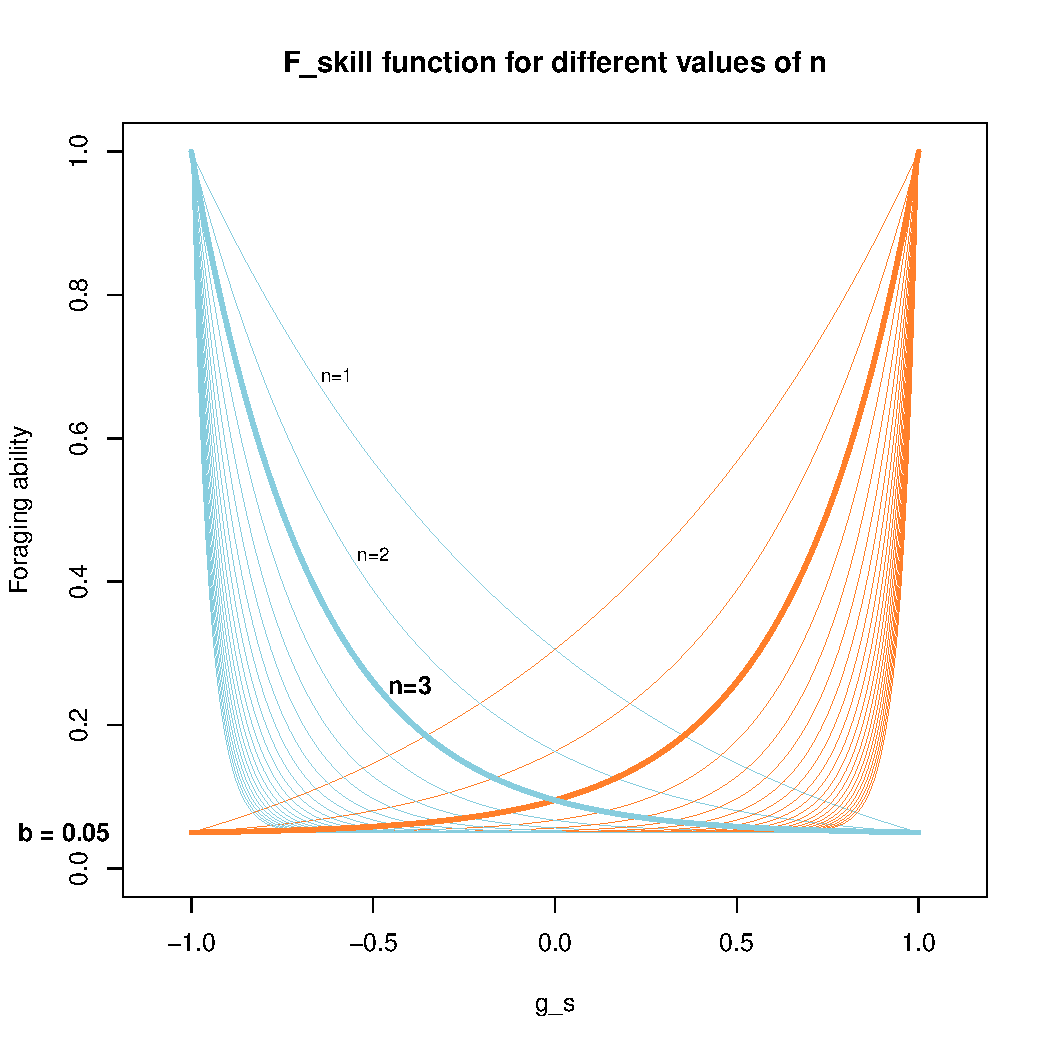
\includegraphics[width=.45\textwidth]{images/f_skill_alpha}
\caption[Fonction d'atteinte des ressources]{Illustration de la fonction d'atteinte des ressources pour différents paramètres $n$}
\label{fig:reward}

\end{figure}

\subsection{Détails des expériences}
\label{sec:exp:detail}
%At this point, it is important to note that the motivation behind this experimental setup is both to stress the population for further analysis as well as providing a flexible and challenging experimental setting that could be re-use to evaluate further versions and variations over the algorithm presented here. To this end, the source code and parameters for all experiments presented in the following is available on-line in the Evolutionary Robotics Database\footnote{Evolutionary Robotics Database: http://www.isir.fr/evorob$\_$db/}. 

Pour mener à bien les simulations nous avons utilisé un ordinateur HP-Z800, une simulation prenant environ 5 min sur un coeur du processeur Intel Xeon cadencé à 2,4Ghz. Les simulations ont été faites à l'aide du simulateur Roborobo programmé en C++ et disponible à l'adresse \url{http://www.lri.fr/~bredeche}.

400 pré-expériences ont été menées en faisant varier les paramètres environnementaux. Ces expériences préliminaires ont été faites sur des durées plus courtes et avec moins d'agents dans le but de paramétrer l'environnement pour obtenir le moins d'extinctions possible en fixant les variables régissant l'exploitation des ressources par les agents (cf. \ref{eq:reward}).

Par la suite 123 expériences ont été faites en paramétrant l'environnement à l'aide des résultats obtenus dans les expériences précédentes. Les détails des paramètres utilisés lors de ces expériences sont donnés en annexes dans le tableau~\ref{tab:params2}.


\chapter{Résultats \& analyse }\label{ch:result}


\section{Diversité et lignées phylogénétiques}
\label{sec:res:trees}

Avant de commencer à analyser les résultats des expériences décrites en~\ref{sec:expspecial} nous avons cherché à caractériser comment les génomes utilisés par les robots se transmettaient lors de l'exécution de l'algorithme mEDEA. 


Pour cela nous avons utilisé une ensemble de données issues de Montanier \& Bredeche (2011). \`{A} partir de ces données nous avons reconstruit les arbres phylogénétiques décrivant la transmission des génomes apparus dans les simulations. Le premier arbre (fig.~\ref{fig:treeA}) montre la grande diversité génétique maintenue à travers les génération par mEDEA. 

En revanche il apparaît clairement sur le second arbre (fig.~\ref{fig:treeB}) que, quelques soient les conditions expérimentales, si les génomes survivant à la fin (ie: utilisés par des robots actifs pendant la dernière itération) sont tous différents, il ne viennent que d'un seul ancêtre commun. Ainsi, même si une lignée apparaît avec une solution quelque peu différente et suffisamment efficace pour se retrouver sur de nombreux robots à la génération suivante, elle finira: (1) soit par se devenir l'ancêtre de tout les autres (2) soit disparaître, remplacée par une autre solution présente en nombre légèrement plus élevé. 

Ce phénomène reflète bien la qualité de l'opérateur de sélection en action dans mEDEA: la sélection se fait totalement aléatoirement. Ainsi, si un génome est initialement plus présent à une génération $t$, la probabilité qu'il se soit sélectionné à la génération $t+1$ est plus élevée ; et ainsi inexorablement les descendants d'un unique ancêtre finiront par être les uniques individus de la population. Sans conditions environnementales adéquates il ne peut apparaître de spéciation.

\begin{figure}[H]
\centering
% 	\hspace{-4cm}
\advance\leftskip-4cm
% 	\advance\rightskip-2cm
\caption[Phylogénétique dans mEDEA]{Transmission des génomes au sein de mEDEA}
\subfloat[Toute les lignées générées pendant une simulation.] {\label{fig:treeA} \includegraphics[width=\textwidth]{images/aRadialTree}}
% 		\hfil
\subfloat[Uniquement les lignées survivantes à la fin de la simulation.] {\label{fig:treeB} \includegraphics[width=.6\textwidth,angle=90]{images/aLinearTree}}

\label{fig:trees}
\end{figure}

\section{Contraintes environnementales et spéciation}

Maintenant que ce passe-t-il dans notre environnement construit pour que l'essaim d'agent autonome se spécialise? L'algorithme est-il capable de faire évoluer des comportements viables? c'est comportement sont-ils spécialisés? se retrouvent-ils sur des espèces différentes?

\subsection{Extinctions}
En premier lieu nous avons cherché à voir si l'algorithme était capable de faire évoluer des contrôleur en mesure de permettre la survie des robots dans notre nouvel environnement. 

Sur les 123 expériences 120 ont généré des contrôleurs ayant permis aux robots de survivre plus de de 300\,000 itérations, soit potentiellement plus de 975 générations. Cela ne fait que $2,43\%$ d'extinctions, ce qui vient confirmer le bon choix des paramètres environnementaux fait en~\ref{sec:exp:detail}.
Les expériences pendant lesquelles des extinctions rapides ont eu lieu ne seront pas analysée, c'est pourquoi le reste des résultats sera commentés d'après ces 120 expériences.


De fa\c con globale la figure~\ref{fig:surviagent} montre qu'assez vite plus de la moitié des agents survivent. Néanmoins il est notable qu'un certains nombre de simulations présentent un nombre assez faible d'agents en vie jusqu'à la dernière itération, nous verrons pourquoi cela dans la section suivant avec l'analyse des comportements <<opportunistes>>.

\begin{figure}[H]
\centering
\includegraphics[width=.75\textwidth]{images/survivingAgents-woDenisity120runs}
\caption[Nombre d'agents survivants]{Nombres d'agents survivants à chaque itération pour les expériences n'ayant pas mené à une extinction rapide.}
\label{fig:surviagent}
\end{figure}

L'algorithme a donc en genéral fait évoluer des contrôleurs adéquats, capable de garder en vie un grand nombre d'individus (près de 70\% de la population).

Partant de ces 120 expériences voyons de plus près les types de stratégies adoptées par les agents.

\subsection{Stratégies}
\label{sec:res:spec}
Maintenant regardons comment se comportent les contrôleurs ayant évolué dans cet environnement. Sont-ils spécialisés sur l'exploitation d'une ressource, des deux ou d'aucune? Pour cela nous avons analysé une à une les 120 expériences sélectionnées dans la section précédente et en avons extrait deux stratégies globales à partir desquelles chaque expérience peut être décrite:

\begin{enumerate}[S1:]\setcounter{enumi}{-1}
\item Des comportements chaotiques, qui utilisent le fait que l'environnement permet aux individus d'être rechargés en énergie lorsqu'ils se <<réveillent>>. Ces comportements peuvent se traduire par un certain nombre de sous stratégies particulières (voir figure~\ref{fig:opportuniste}). Pour simplifier nous les considérerons toutes comme une seule, qualifiée d'\emph{opportuniste}. Ces stratégies se caractérisent par un nombre très faible d'agents en vie, regroupés en petits groupes activés à tour de rôle. \label{itm:chaos}
\item Les agents sont spécialisés dans l'exploitation d'une ressource et l'exploitent en la suivant et en restant proche de celle-ci. Nous utiliserons les indices $B$ et $R$ pour spécifier sur l'exploitation de quelle source (Rouge ou Bleu) le groupe est spécialisé. \label{itm:1spe}
\end{enumerate}

Lors d'une expérience avec mEDEA ces deux stratégies globales peuvent s'enchaîner, coexister et disparaître selon différents schémas évolutionnaire. Ces schémas reviennent à des fréquences différentes dans notre corpus de simulations. Ces schémas et leur fréquence d'apparition parmi l'ensemble des simulations sont décrits dans le tableau~\ref{tab:res:strat} et illustrés par les graphiques de la figure~\ref{fig:evol}.
% \todo{toujours pas fait}

% \begin{enumerate}[schema 1]
% \item	S\ref{itm:1spe}$_X$ uniquement 		(fig.~\ref{fig:evol:1S1quick}) : les stratégies opportunistes se maintiennent toute la simulation. %\lablem{it} 
% \item	S\ref{itm:chaos} uniquement 					
% \item	S\ref{itm:chaos} $\rightarrow$  S\ref{itm:1spe}$_X$ 		(fig.~\ref{fig:evol:chaostoS1})	 	
% \item	S\ref{itm:1spe}$_X$ $\rightarrow$ S\ref{itm:chaos} $\rightarrow$  S\ref{itm:1spe}$_X$ 		(fig.~\ref{fig:evol:1S1to1S1})	
% \item	S\ref{itm:1spe}$_Y$ \& S\ref{itm:1spe}$_X$  $\rightarrow$ S\ref{itm:1spe}$_Y$ \& S\ref{itm:1spe}$_X$ (fig.~\ref{fig:evol:2S1to2S1})
% \item	S\ref{itm:1spe}$_Y$ \& S\ref{itm:1spe}$_X$  $\rightarrow$ S\ref{itm:1spe}$_X$ 	(fig.~\ref{fig:evol:2S1to1S1}) 
% \item	S\ref{itm:1spe}$_X \rightarrow$ S\ref{itm:chaos} $\rightarrow$ S\ref{itm:1spe}$_Y$ 	(fig.~\ref{fig:evol:S1toS1})
% \end{enumerate}


\begin{table}[H]
% \tbl{
	\centering
	\caption[Fréquences des schémas évolutionnaires]{Répartition des différents schémas d'évolution des stratégies obtenues parmi toutes nos expériences (avec $(X,Y)\in\{R,B\}$):}
	\label{tab:res:strat}
	
	\begin{tabular}{lr} 
	% 	\toprule
	\textbf{\'{E}volution des stratégies observées} & \textbf{Pourcentage de cas} \\ \hline
	% 	\colrule
	% 	arena width and length & $1024*530$ pixels \\ 
	% % % 	"free-ride" setup duration & 75 generations \\ 
	%"energy" setup duration & 75 generations \\ 
	S\ref{itm:1spe}$_X$ uniquement 		(fig.~\ref{fig:evol:1S1quick})	& $25,8\%$\\
	S\ref{itm:chaos} uniquement 		(fig.~\ref{fig:evol:chaos})				& $3,3\%$ \\
	S\ref{itm:chaos} $\rightarrow$  S\ref{itm:1spe}$_X$ 		(fig.~\ref{fig:evol:chaosto1S1})	 	& $51,8\%$\\
	S\ref{itm:1spe}$_X$ $\rightarrow$ S\ref{itm:chaos} $\rightarrow$  S\ref{itm:1spe}$_X$ 		(fig.~\ref{fig:evol:1S1to1S1})	& $3,33\%$\\
	S\ref{itm:1spe}$_Y$ \& S\ref{itm:1spe}$_X$  $\rightarrow$ S\ref{itm:1spe}$_Y$ \& S\ref{itm:1spe}$_X$ (fig.~\ref{fig:evol:2S1to2S1})	& $0,83\%$ \\
	S\ref{itm:1spe}$_Y$ \& S\ref{itm:1spe}$_X$  $\rightarrow$ S\ref{itm:1spe}$_X$ 	(fig.~\ref{fig:evol:2S1to1S1}) 	& $11,7\%$ \\
	S\ref{itm:1spe}$_X \rightarrow$ S\ref{itm:chaos} $\rightarrow$ S\ref{itm:1spe}$_Y$ 	(fig.~\ref{fig:evol:S1toS1})		& $2,5\%$\\
	% 	\botrule
	\end{tabular}
	
	\end{table}
	
	
	Si nous regroupons ensembles les schémas se concluant par une stabilisation sur une seule population spécialisée dans l'exploitation d'une ressource, on observe que $92\%$ des simulation se terminent ainsi. Ce qui n'est pas surprenant au regard des résultats observés dans les expériences précédentes reprises en \ref{sec:twosuns}. 
	
	Il est à noter que très souvent cette stabilisation ne s'obtient qu'après une période plus ou moins longue pendant laquelle des stratégies opportunistes occupent l'environnement. La figure~\ref{fig:opportuniste} permets de voir le comportement de certaines de ces stratégies opportunistes plus en détails. Ce sont elles ces stratégies S\ref{itm:chaos} qui sont responsables des expériences pendant lesquelles le nombre d'agents reste assez faible et des valeurs minimales observables sur le graphique de la figure~\ref{fig:surviagent}.
	
	De plus, en raison des observations faites en~\ref{sec:res:trees}, il est très difficile pour une nouvelle stratégie de s'imposer dans une population déjà majoritaire. C'est pourquoi les <<basculements>> d'une stratégie à l'autre (fig.~\ref{fig:evol:S1toS1}), ne peuvent pas avoir lieu sans une période pendant laquelle une stratégie qui avait précédemment le dessus s'éteint, ne laissant plus que quelques groupes de survivants opportunistes qui pourrons être facilement convertis par une stratégie un peu plus efficace. 
	
	%%%%%%%%%%%%%%%%%%%%%%%%%5
	\begin{figure}[H]
	\centering
	\includegraphics[width=.75\textwidth]{images/201129_agentOportunistes_passlifetorchbis}
	\caption[Stratégies opportunistes]{Visualisation de différentes stratégies opportunistes (stratégie~\ref{itm:chaos}). Les robots se suivent par petite groupes de 4 à 5 robots et se réactivent à tours de rôle. Ils usent ainsi de la possibilité offerte aux robots n'ayant pas de génomes à la fin de leur vie d'être réactivés une génération si un autre robot leur transmet un génome. Ici les deux stratégies observées ne se préoccupent pas de l'énergie, l'essentiel est de savoir que d'autres groupes prendront le même chemin et pourront réactiver le groupe n'ayant plus d'énergie. C'est pourquoi il est fréquent de voir des robots suivre une source d'énergie (les robots suivants les flèches rouges), les sources d'énergie leur fournissant un objectif commun, tandis qu'en général ils ne font que longer les murs (parcours des flèches en vert). Ce cas correspond au cas~\subref{fig:evol:chaos} de la figure~\ref{fig:evol}. }
	\label{fig:opportuniste}
	\end{figure}
	%%%%%%%%%%%%%%%%%%%%%%%%%5
	
	De plus, une seule expérience réussie à maintenir deux sous espèces spécialisées dans l'exploitation des deux types de ressources (fig.~\ref{fig:evol:2S1to2S1}) ; tandis que la plupart du temps, ces cas di-morphismes comportementaux ne sont observés qu'au début de la simulation ($11.7\%$ des cas).
	
	% \todo{analyse des repartitions}
	
	Une dernière remarque est qu'il est parfois difficile de classer correctement les stratégies en ne se basant que sur la localisation géographique et $g_skill$. Dans certains cas il est très difficile de savoir si il y a une seule population qui suit la source qu'elle exploite ou si nous avons à faire à un mix de stratégies spécialisés et de stratégies opportunistes. Et si parfois les transitions entre une stratégie spécialisé et un ensemble de stratégies opportunistes sont claires car le nombre d'individus chute de beaucoup et pendant une durée suffisante, elles peuvent parfois être trop rapides pour être per\c cues.  Un outil pour classifier et grouper les différentes stratégies et espèces obtenues est à mettre en place à l'avenir pour permettre une meilleur analyse des simulations.
	
	
	
	Pour résumer : dans la quasi-totalité des cas une seule stratégie se maintient jusqu'à la fin de la simulation. dans ces cas là l'ensemble de la population est spécialise dans l'exploitation d'une ressource particulière et s'y tient. Néanmoins il n'est pas rare que deux sous-espèces spécialisées cohabitent un certains temps, sans que la cohabitation ne dur. \'{A} une exception près, pendant laquelle un dimorphisme pérenne émerge. Dans d'autres rares cas les populations ne se spécialisent sur aucune ressource et adoptent des stratégies opportunistes (cf.~\ref{fig:opportuniste}) basés sur des consensus d'auto-réveils.
	
	%%%%%%%%%%%%%%%%%%%%%%%%%5
	\newcommand{\graphSize}{.65\textwidth}
	\newcommand{\myspace}{.1cm}
	
	\begin{figure}[H]
	% \advance\leftskip-4cm
	\centering
	% \hspace{\leftAdj}
	% \vspace{-4cm}
	\advance\leftskip-4cm
	\advance\rightskip-4cm
	
	\subfloat[ S\ref{itm:1spe}$_B$ $\rightarrow$  S\ref{itm:1spe}$_B$: Dès le début un agent apparaît avoir un comportement adapté et son génome se répand à travers toute la population, qui se stabilise en une population unique spécialisée dans l'exploitation d'une seule ressource (ici B).]{
		\includegraphics[height=\graphSize]{images/S1quick}
		\label{fig:evol:1S1quick}
	}\\
	% 	\hspace{\leftAdj}
	\subfloat[ S\ref{itm:1spe}$_R$ \& S\ref{itm:1spe}$_B$  $\rightarrow$ S\ref{itm:1spe}$_R$ \& S\ref{itm:1spe}$_B$: Deux espèces spécialisées chacune sur l'exploitation d'une ressource, qui se maintiennent durant quasiment toute la simulation. \`{A} la nuance près qu'à la 150\,000e itération, une mutation empêchant les agents présents sur la ressource bleu de prendre cette dernière, se propage suffisamment pour envahir toute la population vivant sur la source bleu. La transmission de cette mutation entraîne une chute clairement visible du nombre d'individus en vie, on peut imaginer que la population use ici en réalité de stratégies opportunistes. Le hasard a fait que dans ce cas précis très vite des mutations ont permis à un certain nombre d'individus de récolter la ressource bleue à nouveau.]{ 
		\includegraphics[height=\graphSize]{images/2S2to2S2}
		\label{fig:evol:2S1to2S1}
	}
	\hspace{\myspace}
	\subfloat[ S\ref{itm:chaos} $\rightarrow$  S\ref{itm:1spe}$_B$: Pendant longtemps seuls quelques groupes d'agents aux stratégies opportunistes survivent, maintenant ainsi le nombre d'agents actifs relativement bas, sans pour autant mener à l'extinction. La prédominance de la couleur orange sur la graphe indique pourtant que les agents suivent bien le soleil orange, mais, tout comme c'est le cas de la stratégie verte dans la figure~\ref{fig:opportuniste}, $g_skill$ ne permet à personne d'exploiter cette ressource. Puis, aux alentours de l'itération 300\,000, une suite de mutations entraînent suffisamment d'individus à suivre l'autre soleil. $g_{skill}$ n'ayant pas muté, la sous-population est déjà apte à exploiter B et va très vite se répandre et être adoptée par l'ensemble de la population.]{
		\includegraphics[height=\graphSize]{images/S0to1S1}
		\label{fig:evol:chaosto1S1}
	}
	
	\phantomcaption
	
	\end{figure}
	
	\begin{figure}[H]
	\ContinuedFloat
	\centering
	\vspace{-4cm}
	\advance\leftskip-4cm
	\advance\rightskip-4cm
	
	\hspace{\myspace}
	\subfloat[S\ref{itm:1spe}$_B \rightarrow$ S\ref{itm:1spe}$_R$: Dans ce cas la population passe d'un seul groupe spécialisé sur l'exploitation d'une ressource, à un seul autre groupe, mais spécialisé sur l'exploitation de l'autre ressource. Il est à noter que ce basculement ne semble pouvoir se produire (et n'a jamais été observé) sans une transition pendant laquelle la majorité des agents actifs pratiquent l'opportunisme. Elle apparaît clairement ici, au alentours de la 10\,000e itération, quand le nombre d'agents actifs diminue, laissant place à une sous-population intermédiaire incapable d'exploiter aucune des deux ressources mais qui permettra de muter correctement $g_{skill}$ et ensuite changer de source.]{
		\includegraphics[height=\graphSize]{images/S1toS1}
		\label{fig:evol:S1toS1}	
	}
	\hspace{\myspace}
	\subfloat[S\ref{itm:chaos} uniquement: tout comme dans le graphe~\subref{fig:evol:chaosto1S1} la première solution à se répandre dans la population est une population opportuniste qui restera cette fois majoritaire jusqu'à la fin de la simulation. Même si les agents semblent suivre le soleil orange, $g_{skill}$ ne leur permet pas de l'exploiter, et même lorsque aux alentours de la 160\,000e itération une mutation semble offrir à certains cette capacité, leur nombre et ou peut-être une mutation avec un impact négatif sur leurs capacités à suivre le soleil, ne suffit pas à fournir les capacités pour convertir le reste de la population ; et la mutation reste masquée par le <<bruit>> généré par les stratégies opportunistes. ]{
		\includegraphics[height=\graphSize]{images/S0toS0}
		\label{fig:evol:chaos}	
	}\\
	\subfloat[S\ref{itm:1spe}$_R$ \& S\ref{itm:1spe}$_B \rightarrow$ S\ref{itm:1spe}$_R$: deux populations spécialisées dans l'extraction des deux sources émergent assez vite, puis le mécanisme observé dans la section~\ref{sec:res:trees} fait qu'au bout d'un certain temps la population sur la ressource la plus exploitée va prendre le dessus et être transmise à l'ensemble des robots.]{
		\includegraphics[height=\graphSize]{images/2S1to1S1}
		\label{fig:evol:2S1to1S1}	
	}
	\hspace{\myspace}
	\subfloat[S\ref{itm:1spe}$_R \rightarrow$ S\ref{itm:chaos} $\rightarrow$ S\ref{itm:1spe}$_R$ : Une première population spécialisée sur l'exploitation de la source rouge apparaît. Puis, aux alentours de la 220\,000e itération, elle est remplacée par une population d'individus aux stratégies opportunistes qui sera à nouveau très vite remplacée par une autre population spécialisée sur $R$.]{
		\includegraphics[height=\graphSize]{images/1S1tochaosto1S1}
		\label{fig:evol:1S1to1S1}	
	}
	\caption[Différents cas de figures]{Dans la partie supérieure du graphique est inscrite la valeur du gène $g_{skill}$ de chaque robot lorsqu'il sélectionne un nouveau génome et entame ainsi une nouvelle <<vie>> (d'une durée de 400 itérations dans le cas présent). Ainsi un point en -0.2 à l'itération 100\,000 signifie qu'un robot a utilisé un génome avec $g_{skill}=-0.2$ à cette itération. La couleur indique la position en $x$ du robot au moment d'utiliser le génome: plus le point est orange plus l'activation se fait proche de la droite de l'environnement (du côté de la source orange), plus le point est bleu plus l'activation s'est faite à gauche (du côté de la source bleu). La partie inférieure résume le nombre de robots actifs en tout pendant l'itération. }
	\label{fig:evol}
	\end{figure}
	% \todo{mettre un graphe rouge vers bleu}
	
	
	
	
	%%%%%%%%%%%%%%%%%%%%%%%%%5
	\subsection{Espèces}
	Pour analyser les relations de filiation entre les individus utilisant différentes stratégies et pour comparer avec les résultats observés en~\ref{sec:res:trees} nous avons analysé comment étaient transmis les génomes dans deux cas particuliers de notre expérience :
	
	\begin{itemize}
	\item Un cas avec une seule population spécialisée sur une seule source (fig.~\ref{fig:evol:1S1quick}),
	\item Le cas avec deux populations spécialisées sur deux sources (fig.~\ref{fig:evol:2S1to2S1}).
	\end{itemize}
	
	% Si en règle générale, comme le montre le tableau~\ref{tab:res:strat}, les simulations vont se stabiliser à un équilibre composé d'une seule stratégie, les graphiques~\ref{fig:ancestors} montrent que dans les cas ou deux sous-population émergent, ces dernières sont bien issues de deux ancètres différents. 
	
	
	%%%%%%%%%%%%%%%%%%%%%%%%%5
	\begin{figure}[H]
	\subfloat[Pour une simulation de type de celle de la fig.~\ref{fig:evol:1S1quick}]{\includegraphics[width=6cm]{images/ancestors1species.png}}
	\hspace{.2cm}
	\subfloat[Pour une simulation de type de celle de la fig.~\ref{fig:evol:2S1to2S1}]{\includegraphics[width=6cm]{images/ancestors2species.png}}
	\caption[Pères fondateurs]{Nombre d'ancêtres à l'origine des individus actifs pendant la dernière itération. Attention ici l'échelle est en générations, soit 400 itérations (300G = 120\,000it).}
	\label{fig:ancestors}
	\end{figure}
	%%%%%%%%%%%%%%%%%%%%%%%%%5
	
	Si on remonte suffisamment dans le temps et que l'on observe le nombre d'ancêtres à l'origine des individus de la dernière génération pour une simulation du type de celle présentée à la figure~\ref{fig:evol:1S1quick}, ont remarque, tout comme nous l'avions déjà observé dans les expériences analysées en~\ref{sec:res:trees}, que les génomes présents ne descendent que d'un seul ancêtre commun, qu'ils sont donc de la même espèce. En revanche si l'on observe les ancêtres des individus de la dernière génération d'une simulation ou deux stratégies sont apparues (fig.~\ref{fig:evol:2S1to2S1}) il y a bien deux individus, ancêtres des deux espèces différentes ainsi crées.
	
	
	Contrairement aux cas présentés en~\ref{sec:res:trees} les cas ou deux stratégies apparaissent présentent bien deux lignées génétiques différentes, stable sur la durée.
	
	
	\chapter{Discussion \& perspectives }\label{ch:discussion}
	
	Est-il possible de spécialiser une population d'agents autonomes par le biais d'une évolution \emph{open-ended}, en ne comptant que sur les capacités d'auto-organisation de l'essaim, les contraintes environnementales et les phénomènes de spéciation qui apparaissent lors de processus évolutifs?
	
	Nous avons montré que oui, cette spécialisation est possible (cf. fig.~\ref{fig:evol:2S1to2S1}), et qu'elle est bien corrélée avec une divergence génétique des deux sous-populations en deux sous espèces (fig.~\ref{fig:ancestors}. Néanmoins, la majeure partie du temps, cette spéciation n'est que transitoire (fig.~\ref{fig:evol:2S1to1S1}). Les cas pendant lesquels elle se maintient sur la durée sont exceptions et le fruit de conditions initiales de l'expérience particulières et propices.
	La spéciation possible que l'on observe est allopatrique. Pour qu'émerge une spécialisation capable de perdurer sur le long terme même lorsque les populations interagissent, il nous faudra probablement contraindre l'environnement. 
% 	pour qu'une spéciation sympatrique puisse avoir lieu. 
	
	Une première piste à explorer est d'ajouter une pénalisation lorsque trop partagent la même ressource. En effet, dans les conditions actuelles, les deux ressources sont considérées comme illimitées. Il est donc évident qu'il n'y a aucun gain à être spécialisé sur \emph{les deux} ressources. Il suffit que tous les individus se spécialisent sur l'extraction d'une seule pour que tous survivent. C'est pourquoi nous sommes entrain de tester un cas dans lequel lorsque le nombre d'agents qui exploitent une même ressource augmente, la disponibilité de cette ressource diminue (et ne peut donc fournir tout le monde, voir la figure~\ref{fig:densite}).
	
	De plus, si en règle général la population finit par atteindre un effectif assez élevé et que les extinctions sont rares (adaptation efficace aux contraintes), il arrive encore trop souvent que des solutions <<opportunistes>> se répandent. Ces dernières témoignent de la capacité des systèmes \emph{open-ended} à profiter de l'environnement et trouver des solutions auxquelles le concepteur n'aurait pas pensé. Mais si elle permettent de conserver un nombre d'individu en vie minimum et limiter les extinctions, elles peuvent parfois masquer certains phénomènes intéressants.
	
	
	%%%%%%%%%%%%%%%%%%%%%%%%%5
	\begin{figure}[H]
	\centering
	\includegraphics[width=.6\textwidth]{images/densite}
	\caption[Pénalisation par la densité]{La quantité d'énergie reçue par les agents lorsqu'ils atteignent une source diminue quand le nombre d'agents $n$ présents sur cette ressource (noté \emph{\#harvester} sur le graphique) augmente.}
	\label{fig:densite}
	\end{figure}
	%%%%%%%%%%%%%%%%%%%%%%%%%5
	
	Pour terminer, le tableau~\ref{tab:res:strat} montre que des conditions initiales peuvent émerger beaucoup de schémas évolutionnaires différents. Il est par exemple possible d'observer la disparition d'une espèce qui paraissait avoir trouvé une bonne stratégie. Parfois cette extinction n'est que passagère et la même stratégie réapparaît quelque temps après (fi.~\ref{fig:evol:1S1to1S1}) ; parfois après l'extinction la population se spécialise sur l'extraction d'une autre source (figure~\ref{fig:evol:S1toS1}). Quoi qu'il en soit cela pose la question de la stabilité évolutionnaire, au sens de Maynard-Smith, de nos stratégies, stabilité qu'il nous faudra à l'avenir étudier.
	
% 	
	\newpage
% 	
% 	
	\begin{itshape}
		\small
		\paragraph{Remerciements}
	
		On commence tout jeune à écouter avec envie les profs qui nous racontent milles histoires sur le monde qui nous entoure et qu'on regarde d'en bas un peu craintivement. Puis on finit par comprendre ces histoires et faire quelques centimètres de plus, alors on nous en raconte d'autres. On finit aussi par les comprendre, par prendre encore quelques centimètres et \c ca recommence.
		Puis un jour, en pleine lecture d'une histoire un peu plus corsée que les autres, pleine de concepts émergents aux motivations un peu trop stochastiques voir floues pour être vraiment honnêtes, qui cherchent une bio-inspiration passagère dans l'espoir vain de sauver une belle heuristique enfermée dans des abimes de bruit non paramétrique, on lève les yeux du polycopié froissé et griffonné de signes obscures qui a remplacé le cahier de fran\c cais avec sa marge rose et ses interlignes ; et on remarque que le prof n'est plus au tableau mais à coté et qu'il demande avec tout le sérieux du monde "tu crois que \c ca marcherait?". Si je crois que \c ca marcherai? mais quelle question, aucune idée. Surpris on sort de l'étrange salle pleine de barbelus se grattant la tête dans laquelle se déroulait la scène et on jette un coup d'oeil dans la cour pour essayer d'y trouver le bureau des CPEs... il a disparu. Tout comme il impossible de retrouver la fois ou les gens qui s'en occupent ont décidé qu'on écrirait plus centimètres, mais kilogrammes. Alors je vais aller demander à la maîtresse, elle doit savoir.
	% 	' celle que les profs du début avaient écouté avant de nous les racontées à nous. Et celle-là aussi on fini par les comprendre. Alors là les profs commencent à nous demander de regarder avec eux le monde qu'ils observent depuis si longtemps pour qu'ils puissent le comprendre mieux encore et raconter de nouvelles histoires à son sujet à d'autre profs, à d'autres élèves. Là on comprend d'un coup beaucoup moins vite, mais c'est pas grave, parce que l'essentiel surtout, c'est qu'on fini par tutoyer ses profs (ou pas), l'écart d'âge étant chaque fois moins important. Et puis quand on comprend, on comprendre avec eux. Et sans vraiment s'en rendre compte on devient un peu profs nous même. 
		En poussant jusqu'à la maternelle on réalise qu'en s'allongeant en travers du bac à sable, on peut atteindre les deux bouts en écartant les bras. Et en y regardant de plus près on comprend même pourquoi les fourmis qui nous grattaient la cheville 20 ans auparavant se suivaient si fidèlement pour aller de l'herbe jusqu'à la sucette qu'on avait lâchée malencontreusement et qui avait fait coulée pas mal de larmes. Vraiment étrange. D'autant que la maîtresse ne semble avoir aucune envie de répondre à la question. En fait on dirait que c'est elle qui écoute. Et sans même l'avoir pensé on s'entend raconter de longues minutes d'histoires, toutes celles qu'on a vécues, qu'on nous a apprises et racontées, après que chaque années on ait fini par arriver chez <<les grands>>. C'est donc ça. On doit être presque grand alors. On a des histoires à raconter. Les mêmes qui déjà à l'époque, nous avaient fait briller les yeux entre deux jets de cartouche d'encre turquoise, les mêmes mais quelques maladresse et deux ou trois  détails croustillants en plus.
		
	% 	Ces maitresses qui n'ont pas changées, et qui nous reconnaissent encore.
	
		Je remercie tous les encadrants, enseignants, professeurs, qui m'ont un jour raconté que le monde autour de moi était beau ou intéressant, ou les deux si tant est que cela fait une différence, et que \c ca valait la peine de s'y pencher de temps en temps. Merci.
	
	% 	Je ne citerais pas tous les noms, sait-on jamais, il faut en garder au cas ou l'histoire continue un ou deux crans plus loins. 
		
		Nominativement je remercierai quand même les gens qui ont contribué à l'élaboration de ce présent rapport: 
	
		\emph{Fabien Laborie} pour la figure~\ref{fig:speciation}: elle respire le bonheur et l'herbe de Montchabout ces fleurs, tant qu'on ne souhaite qu'y allonger ses souvenirs pour admirer les étoiles,
	
		\emph{Nicolas Bredèche}, dont les idées et la méthodologies sont la structure et la substance véritable de ce rapport sur lesquels je n'ai fait que clouer des mots (mals orthographiés) et quelques lignes de code. %En esperant que 
	
		Les autres membres de l'équipe TAO, qui sont toujours de bons conseils, notamment les petits jeunes du bureau d'à côté, Nico et Seb pour l'après-midi consacrée à me trouver une fonction digne de ce nom, et Jean Marc sans qui les points noirs sur l'écran seraient encore entrain de flâner tranquillement entre deux adresses de mémoire vive.
		
		Et je tiens aussi à remercier \emph{Elisabetta Zibetti}, parce qu'elle me supporte depuis maintenant le début (du master), et que c'est pas encore fini (enfin le master espérons que si).
	
		\end{itshape}
% % 	\twocolumn
	
	\bibliographystyle{apalike}
	\addcontentsline{toc}{chapter}{Bibliographie}
	%%\bibliography{/home/simon/www/simon.bib,/home/simon/evorob/Doc/bib/nicolas.bib,/home/simon/evorob/Doc/bib/jeanmarc.bib}
	\bibliography{/home/simon/projects/TAO/evorob/Doc/bib/simon,/home/simon/projects/TAO/evorob/Doc/bib/nicolas,/home/simon/projects/TAO/evorob/Doc/bib/jeanmarc}
	
	\appendix
	\chapter{Appendices A}
	
	
	\section{Algorithme}
	Description de l'algorithme mEDEA, exécuté localement sur chaque agent :
	
	\vspace{-5pt}
	\begin{algorithm}[H]
	\caption{minimum Environnement Driven Evolutionnary Algorithm}          % give the algorithm a caption
	\label{alg:medea} 
	{\small
	\begin{algorithmic}
	\STATE $genome$.randomInitialize()
	\WHILE{forever}
	\IF { $genome$.notEmpty() }
	\STATE agent.load($genome$)
	\ENDIF
	\FOR { $iteration$ = 0 to $lifetime$ }
	\IF { agent.energy $>$ 0 and $genome$.notEmpty() }
	\STATE agent.move()
	\STATE broadcast($genome$)
	\ENDIF
	\ENDFOR
	\STATE $genome$.empty()
	\IF { \textit{genomeList}.size $>$ 0 }
	\STATE $genome$ = applyVariation($select_{random}$(\textit{genomeList}))
	\ENDIF
	\STATE \textit{genomeList}.empty()
	\ENDWHILE
	\end{algorithmic}
	}
	\caption{minimal Environment-driven Distributed Evolutionnary Adaptation Algorithm}
	\end{algorithm}
	
	
	\section{Caractéristiques des expériences}
	
	\subsection{Détails des paramètres}	
	\label{ann:param}
	\begin{table}[H]
	% \tbl{\subsection{par}
	\caption{Paramètre des agents.}
	\label{tab:params1}
	
	\begin{tabular}{cc} 
	% 	\toprule
	\textbf{Paramètre} & \textbf{Valeur} \\ \hline
	% 	\colrule
	% 	arena width and length & $1024*530$ pixels \\ 
	% % % 	"free-ride" setup duration & 75 generations \\ 
	%"energy" setup duration & 75 generations \\ 
	durée d'une simulation & 1000 génération\\
	durée de vie d'un génome & 400 iterations \\ 
	taille de la population & 100 agents\\ 
	portée des capteurs de proximité & 64 pixels \\ 
	porté du signal radio & 32 pixels \\ 
	vitesse de rotation & 0.52 rad/s \\ % 30deg/step \\
	vitesse de translation & 2 pixels/step \\ 
	longueur du génome & 89 valeurs réelles (87 poids + $\sigma$ + $g_{skill}$) \\ 
	opérateur de mutation & mutation gaussienne de paramètre $\sigma$ \\ 
	$\sigma_{minValue}$ & 0.01\\ 
	$\sigma_{maxValue}$ & 0.5\\ 
	$\sigma_{initialValue}$ & 0.1\\ 
	$\alpha$ (ie. paramètre de mise à jour de $\sigma$ ) & 0.35 \\
	% 	\botrule
	\end{tabular}
	
	\end{table}
	
	\begin{table}[H]
	
	\caption{Paramètres de l'environnement}\label{tab:params2}
	\begin{tabular}{cc} 
	% 	\toprule
	\hline
	\textbf{\textit{Environnement à deux sources:}} & \\ 
	\hline
	\hline
	% 	\colrule
	% 	sources d'énergie & 2 \\ 
	taille d'une source d'énergie & 40 pixels de rayon\\ 
	% 	food item regrow delay & btw 400 and 4000 steps (see text)\\ 
	<<teneur énergétique\footnote{ie. énergie fournie par $1$ fruit pris en entier}>> & 400 unité d'énergie \\ 
	consommation énergétique de l'agent & 1 unité énergétique par itération\\ 
	niveau d'énergie maximal de l'agent & 1000 unités énergétiques \\ 
	niveau d'énergie initial & 1600 unités énergétiques\\ 
	durée d'attente \emph{off-line} & 1000 itération + $(x\sim\mathcal{U}(0,400))$\\ 
	
	% 	\botrule
	\end{tabular}
	
	\end{table}
	
	
	% \subsection{Réglage de l'opérateur de mutation}
	
	% L'opérateur de mutation utilisé 
	
	
	
	\subsection{Fonctions régissant les capacités de récolte des agents}
	
	Fonction définissant l'énergie récolté par un agent $i$ à l'itération $t$ sur la ressource $Q$. Il est à noter qu'ici apparaît la pénalisation par la densité qui n'a pas été utilisée dans les expériences présentées ici :
	
	\begin{equation} 
	F_{rwd,t}(i,Q) = f_{skill}\left(g_{s,i},T_Q\right)\times d_{penality}\left(h_{Q,t}\right)\times \alpha
	\end{equation}\label{eq:reward}
	
	\begin{subequations}\label{eq:skill}
	
	Fonction définissant la proportion d'énergie récoltée par un agent $i$ suivant la valeur de $g_{skill}$ en fonction des paramètres environnementaux $(n,b)$ :
	\begin{align}
	f_{skill}(g_{s,i},type_Q)= {e^{n*g_{s,i}*t_Q}+C(b,n) \over {e^{n}+C(b,n)}},\\
	C(b,n) = \frac{(be^{n} - e^{-n})}{(1-b)}.
	\end{align}
	
	\end{subequations}
	
	Where :
	\begin{itemize}
	\item $i$ the agent,
	\item $t$ the iteration of the simulation,
	\item $ d_{penality}(h_{Q,t}) =  1 - \frac {h_{Q,t}} {nrobots} $
	% \item $ f_{skill}(g_{s,i},type_Q)= {\left(e^{n*g_{s,i}*t_q}\right)+C(b,n) \over {e^{n}+C(b,n)}}$
	\item $h_{Q,t} \in [0, n -1]$ the number of robot harvesting $Q$ at $t$ 
	\item $g_{s,i} \in [-1,1]$ the value of the gene for the foraging skill of $i$,
	\item $T_Q\in \{-1,1\}$ the type of the resource Q
	\item $\alpha$ the energetic value of a given fruit on a given source
	% \item $ C(b,n) = {(be^{n} - e^{-n} )\over{(1-b)}} $
	\end{itemize}
	
	
	% \printindex
	\end{document}
